\begin{frame}{Was ist ein Embedded System?}
	Der Ausdruck embedded system bezeichnet einen Computer, der in einem technischen Kontext eingebettet ist. \cite{wikiEmbedded}
	\begin{flushright}
		Nach Wikipedia
	\end{flushright}
	
	Was macht ein Embedded System speziell \cite{embeddedSpecials}
	\begin{itemize}
		\item Echtzeit
		\item Grösse
		\item Kosten
		\item Zeit
		\item Zuferlässigkeit
		\item Sicherheit
		\item Energy
		\item Langlebigkeit
	\end{itemize}
\end{frame}

\begin{frame}{kleines Embedded System}
	was mit uC
\end{frame}

\begin{frame}{grosses Embedded System: ATLAS/LHC/CERN}
	\begin{center}
		\begin{tabular}{cc}
			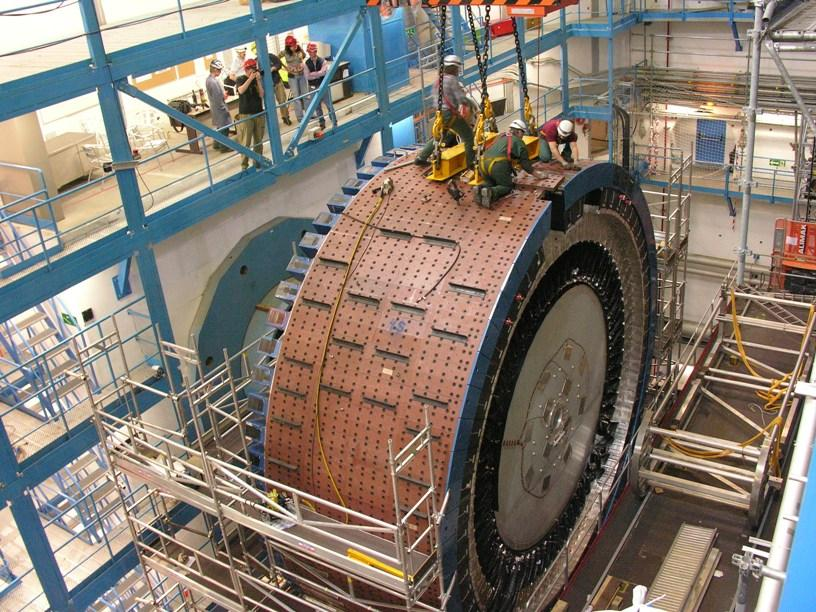
\includegraphics[height=4cm]{res/ATLAS_Tile_Calorimeter} &  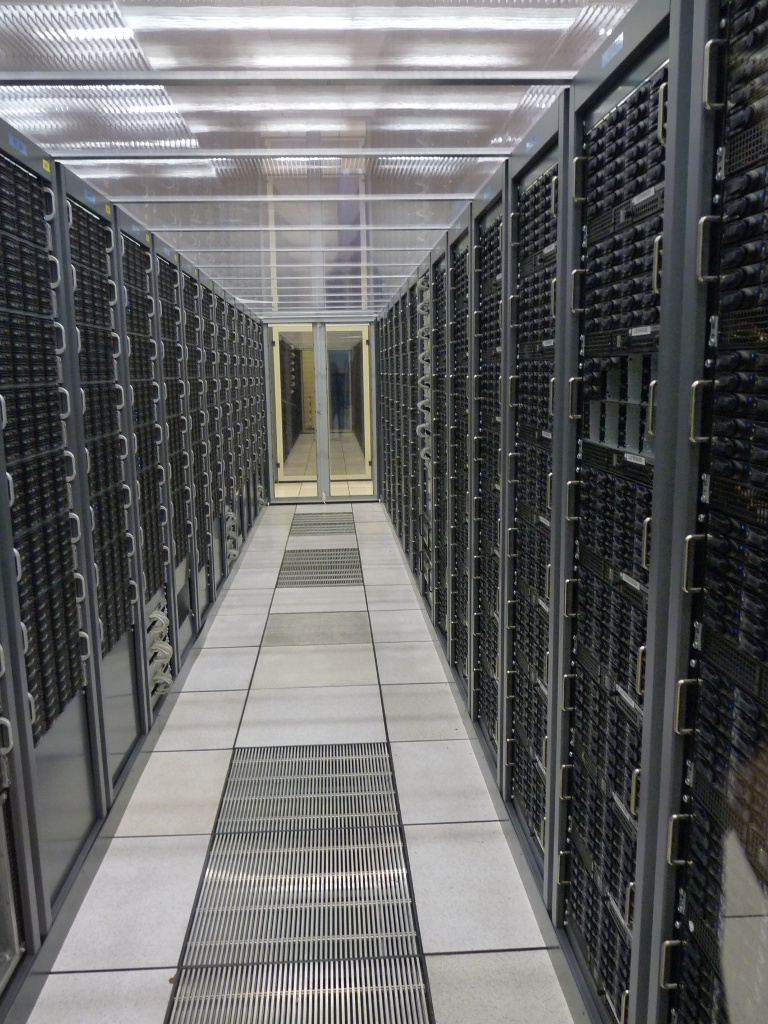
\includegraphics[height=4cm]{res/CERN_server.jpg} \\ 
			cc-by-sa-2.0 Argonne National Laboratory & cc-by-sa Urs Fässler \\
		\end{tabular} 
	\end{center}
	\begin{itemize}
		\item Sensor produziert 1 petabyte Daten pro Sekunde
		\item Systems verarbeitet dies auf etwas mehr als 100 MB pro Sekunde \cite{wikiAtlas}
		\item Verarbeitung auf eigenen 20'000 Server und Grid \cite{wikiCernServer}
	\end{itemize}
\end{frame}

\begin{frame}{prototypisches GNU/Linux Embedded System}
	Raspberry PI
	BeagleBone
\end{frame}
	
